\chapter{Exemple d'application du langage}

PUBG est un jeu vidéo sortit en 2017 avec des millions de joueurs à travers le globe. Développé par PUBG Corporation (filiale de Bluehole, Inc. ou plus récemment de Krafton Game Union) en 2017 c'est un des premiers jeu standalone permettant à ses joueurs de participer à un "last man standing game" suivi de prêt par Fortnite (Epic Games). Ces deux jeux ont été les deux premiers standalone à populariser le Battle Royale et à le mettre à la portée de tous sans devoir développer ou installer des mods dans des jeux existants.

\section{L'origine du Battle Royale}
Le Battle Royale trouve ses racines dans le roman Battle Royale et son adaptation cinématographique. Un programme militaire de simulation de combat prend place da ns une République socialiste d'Extrême Orient complètement coupée du monde extérieur sans aucun droits civiques et extrêmement stable politiquement. Le programme consiste à un tirage au sort annuel de 50 classes de troisième qui sont déplacées chacune vers une zone de combat. Au début de l'expérience tous les élèves sont réunis afin d'obtenir un briefing rapide de l'événement et se voient attribuer un sac contenant un objet (allant d'une arme à feu, à une arme blanche, à une fourchette ou une corde de luth). Ils sont ensuite livrés à eux-mêmes dans une zone donnée en ayant pour seule information : aucune règle n'est imposée et un seul survivant par groupe pourra être gagnant de l'expérience les autres devront être exterminés par n'importe quel moyen à disposition. Le champion obtient le droit de vivre aux frais de l'État pour le reste de ses jours et la reconnaissance comme Héros du pays.

\section{La naissance de la popularité du Battle Royale}
L'intérêt pour le principe du Battle Royale n'explose que plus tard avec le succès de la saga Hunger Games mettant en place l'histoire de Katniss Everdeen, une jeune adulte qui participe de son plein gré aux Hunger Games. Dans un État totalitaire séparé en castes regroupées dans des districts, deux enfants et/ou adolescents sont choisis au hasard dans chaque district afin de devenir les Tribus. Ils sont alors réunis à la capitale et lâchés dans une arène afin de participer à une télé-réalité de match à mort diffusée partout dans le pays.
Son succès a amené les développeurs du jeu Arma II à créer un mode de jeu basé sur les mêmes règles. Ce mode sera alors appelé DayZ et deviendra par la suite un jeu standalone. Un mode voit également le jour : Battle Royale. Développé par Brendan Greene pour Arma II et ensuite Arma III, ce mode gagne suffisament en popularité pour que celui-ci donne naissance au projet de jeu PlayerUnknown's Battlegrounds (PlayerUnknown étant le pseudonyme en ligne utilisé par Brendan Greene).

\section{Les règles de PUBG}
Un avion parcours une ligne droite sur une carte, les 100 joueurs de la partie doivent sauter de cet avion afin d'être parachutés à l'endroit de leur choix à condition qu'il soit à portée. Une fois arrivés au sol, les joueurs partent à la recherche d'armes et d'équipement dans des bâtiments et doivent s'entretuer jusqu'à ce qu'un seul joueur ne soit vivant et gagne ainsi la partie (il est également possible de jouer en duo ou en squad de 4 joueurs ou la dernière équipe debout devient gagnante). Afin de limiter la durée d'une partie, une zone circulaire est définie sur la carte une fois que tous les joueurs ont atterri et celle-ci se réduit par étapes au cours de la partie. Les joueurs en dehors de la zone subissent une certaine quantité de dégâts toutes les secondes s'ils restent en dehors du cercle et ces dégâts augmentent au fur et à mesure que le cercle se resserre.

\section{Les Battle Royale dans le monde du jeu vidéo}
Ces dernières années une quantité astronomique de Battle Royale voit le jour dans le jeu vidéo. De Fortnite (Epic Games) à PUBG, en passant par Apex Legends (Respawn Entertainement), Ring of Elysium (Tencent Games) pour ne citer que les plus importants. Des dizaines de jeux voient le jour ou se réinventent afin de coller à la mode des Battle Royale. Les plus grandes licences de FPS (First Personal Shooters) s'alignent également à cette mode, c'est ainsi que voient le jours les modes de jeu Z1BR (H1Z1), Firestorm (Battlefield V), Blackout (Call of Duty Black Ops IV). Mais cette offre répond à une demande phénoménale du public pour ce mode de jeu qui s'impose dans le marché à la même place que le type de jeu MOBA (Multiplayer Online Battle Arena) qui était grand favoris du public depuis une dizaine d'années à travers les jeux League Of Legends ou Dota 2. Avec le temps les Battle Royale tentent de se réinventer et de trouver de nouveaux publics en gardant le principe de Battle Royale mais en apportant d'autres univers. C'est ainsi que naissent Last Tide et son univers aquatique immergé, Fall Guys : Ultimate Knockout et son univers colorés où de petits personnages à la physique étrange se battent pour une couronne, Cuisine Royale, qui était à l'origine une blague de développeurs mais qui a rencontré un succès, dans lequel les personnages se battent à l'aide d'ustensiles de cuisine.

\section{Représentation d'une partie des mécaniques de PUBG}
\subsection{Les données}
Les données concernant les objets de PUBG sont compliquées à trouver.
Cependant certains site internet se sont spécialisés dans le \emph{mining} d'informations à partir des fichiers du jeu.
C'est le cas du \emph{Gamepedia} spécialisé pour PUBG (\url{https://pubg.gamepedia.com/}).
C'est un Wiki régulièrement mis à jours et possédant assez d'informations pour permettre de modéliser des objets du jeu accompagnés de leur caractéristiques.
Les données sont souvent sujettes à modifications au fur et à mesure des mises à jours du jeu.
Cependant l'exactitude des données n'a pas une importance primordial dans le travail présent.


\subsection{Le profil}
Les stéréotypes présents dans Game Genesis permettent de classifier les \emph{Mechanics} pour la rédaction d'un GDD.
Afin de mieux comprendre le fonctionnement de Game Genesis nous avons extrait une partie du profil dans la Figure~\ref{fig.racine_stereo}.
Cette partie du profil inclue les stéréotypes qui sont utilisés dans les exemples présentés dans la suite du chapitre.
De nombreux attributs ont été rajoutés dans les stéréotypes. 
ceux-ci correspondent aux attributs qui auraient pu être ajoutés par un \emph{game designer} dans le profil
Ajouter des attributs dans le profil permet d'automatiser la présence des attributs dans les classes créées à partir du profil UML par l'héritage.
\begin{figure}[H]
    \centering
    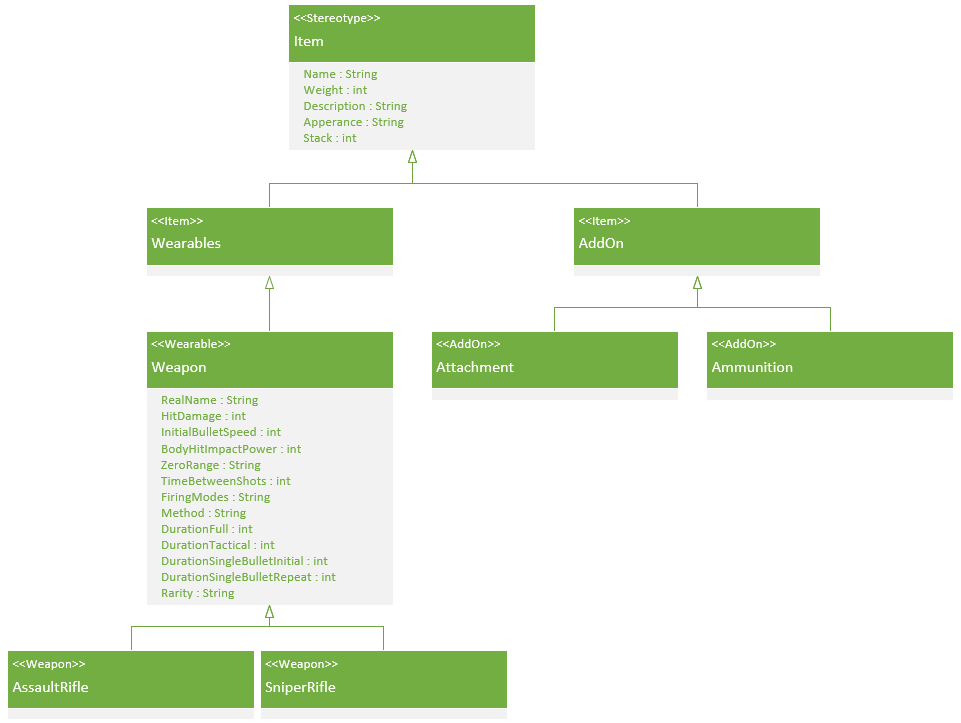
\includegraphics[width=14cm]{10_img/chap6/root(stereotypes).PNG} 
    \caption{Racine des stéréotypes concernés par l'exemple}
    \label{fig.racine_stereo}
\end{figure}

\subsection{La modélisation d'un joueur armé}

\begin{figure}[H]
    \centering
    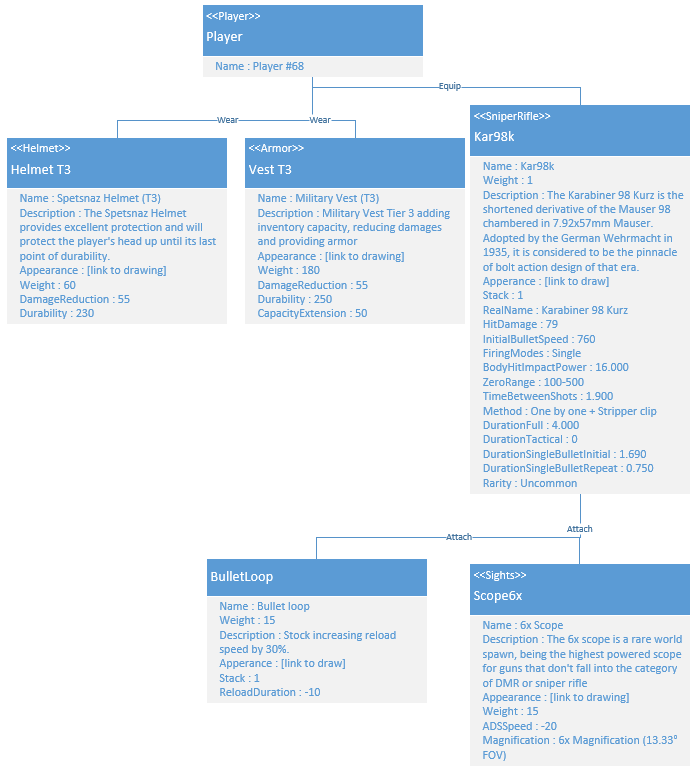
\includegraphics[width=14cm]{10_img/chap6/player68.PNG} 
    \caption{Exemple de modélisation d'un joueur avec son arme}
    \label{fig.player+weapon+equip}
\end{figure}

Dans la Figure~\ref{fig.player+weapon+equip} nous présentons la modélisation d'un joueur.
Celui-ci est équipé d'un casque Tier3 et d'une veste T3. 
Il est armé d'un sniper de type Kar98k lui même équipe d'une lunette x6 et d'une ceinture de munitions.

Comme décris dans la Section~\ref{sect.gg_what} nous avons utilisé des classes afin de représenter les éléments du jeu, alors que des associations entre classes représentent les interactions entre les éléments.
Sur ces classes et associations nous avons appliqué les stéréotypes du profil UML afin de pouvoir classifier et spécialiser les différents éléments modélisés.



\subsection{La modélisation d'une attaque d'un joueur sur un autre}
\begin{figure}[H]
    \centering
    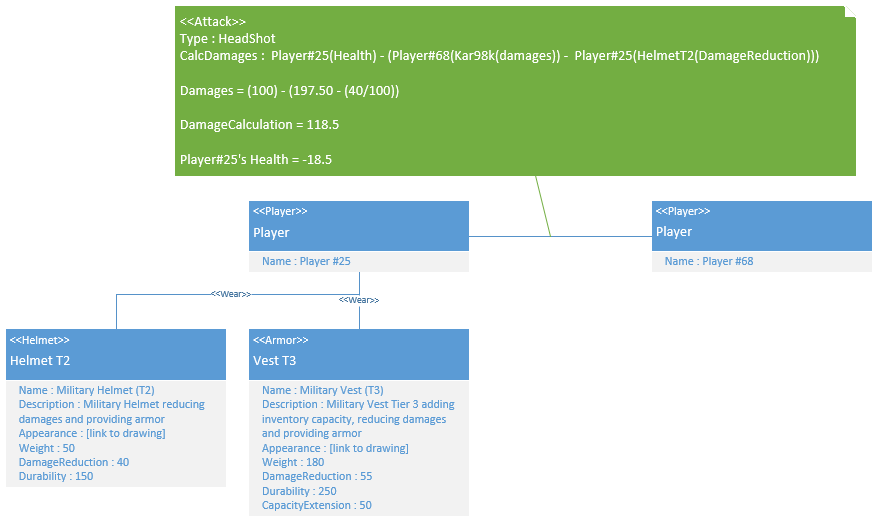
\includegraphics[width=14cm]{10_img/chap6/attack.PNG} 
    \caption{Exemple d'interaction <<~Player68 <<attack>> Player25~>>}
    \label{fig.attack}
\end{figure}

Dans la Figure~\ref{fig.attack} nous représentons un joueur qui en attaque un autre.
L'élément <<~Player68~>> est celui modélisé dans la section précédente.

Le \emph{Game designer} a modifié le stéréotype <<~attack~>> afin que celui-ci comprenne le calcul des dégâts d'un joueur sur un autre.
Afin de calculer ces dégâts nous avons besoin d'un certain nombre d'informations.
Dans un FPS il est possible d'avoir plusieurs types de dégâts en fonction de l'emplacement de l'attaque.
C'est le cas dans PUBG qui différencie les dégâts en trois types : tête, torse et autres.
Ensuite le calcul des dommages s'effectue en prenant en compte les protections portées par le joueur adverse.
Afin d'exprimer le calcul des dégâts nous avons mis en place une formule :

\begin{equation}
\begin{split}
Damages& = Attacker(Weapon(Damages(Type(Value)))\\
Protection& = Defender(Protection(DamageReduction))\\
Calcul& = Defender(health) - (Damages - Protection)
\end{split}
\label{calc.damages}
\end{equation}

Nous retrouvons cette formule de calcul dans la Figure~\ref{fig.attack}.
Elle est présente dans l'association entre les deux joueurs sur laquelle un stéréotype <<~Attack~>> est appliqué.
On considère alors que le \emph{game designer} a modifié le stéréotype dans Game Genesis afin que toutes les actions d'attaque soient régies par cette formule.

Dans cette figure il est spécifié que le joueur <<~Player68~>> effectue un tir à la tête sur le joueur <<~Player25~>>.
Le calcul des dommages renvoie un résultat de 118.5 points de dégats.
Le joueur <<~Player25~>> ne possède cependant que 100 points de vie (\emph{Health}).
On peut donc considérer qu'à la suite de cette action d'attaque, le joueur <<~Player25~>> est éliminé car mort.
Ceci peut être exprimé par les contraintes suivantes :

\begin{table}[H]
\footnotesize
\begin{framed}

    Player(health) : is max 100.\\
    (IF Player(health) < 0)\\
    \{\\
    IF Gamemode is "solo" ==> Player is dead and eliminated.\\
    IF Gamemode is "duo" OR "squad" ==> Player is knocked.\\
    \}
    
\end{framed}
\end{table}

\section{Conclusion}
